%!TEX root = edance.tex
%%%%%%%%%%%%%%%%
%  CHAPTER 10  %
%%%%%%%%%%%%%%%%
\chapter{Complete MOS Small-Signal Model}
\graphicspath{{./figs_mos_ss_ac/}}
%%%%%%%%%%%%%%%%%%%%%%%%%%%%%%%%%%%%%%%%%%%%%%%%%%%%%%%%%%%%%%%%%%%%%%%%%%%%%%%%%%%%%%%%
%%%%%%%%%%%%%%%%%%%%%%%%%%%%%%%%%%%%%%%%%%%%%%%%%%%%%%%%%%%%%%%%%%%%%%%%%%%%%%%%%%%%%%%%
%                                   SECTION 10.1                                       %
%%%%%%%%%%%%%%%%%%%%%%%%%%%%%%%%%%%%%%%%%%%%%%%%%%%%%%%%%%%%%%%%%%%%%%%%%%%%%%%%%%%%%%%%
%%%%%%%%%%%%%%%%%%%%%%%%%%%%%%%%%%%%%%%%%%%%%%%%%%%%%%%%%%%%%%%%%%%%%%%%%%%%%%%%%%%%%%%%
\section{Chapter Preview}
In this chapter we make amends for ignoring charge storage effects in the MOS transistor.  In particular, we focus on the MOSFET capacitance in the saturation regime, including the Gate-Source $C_{gs}$, Gate-drain $C_{gd}$, and drain/source to bulk $C_{db}$ and $C_{sb}$.  This will result in a complete \emph{four terminal} MOS small-signal model.  
%%%%%%%%%%%%%%%%%%%%%%%%%%%%%%%%%%%%%%%%%%%%
A more subtle effect comes from the so-called ``Back-Gate Effect", or how the threshold voltage can be modulated by a source-body bias.  We will model this in the small-signal AC circuit by introducing a back-gate transconductance.  This will result in the complete \emph{four terminal} MOS small-signal model.  This model will be used extensively throughout the rest of this book.
%
%\subsection{What we’ve ignored…until now!}
%
%\begin{figure}[tb]
%\begin{center}
%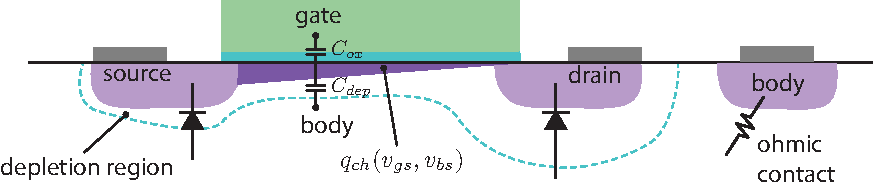
\includegraphics[width=.75\columnwidth]{mos_backgate}
%\end{center}
%\caption{mos backgate} \label{fig:}
%\end{figure}
%
% The fourth terminal of the MOSFET is the body of the transistor
% The junctions of the transistor form pn-junction diodes,and naturally  this introduces parasitic capacitance from source and drain to the body or bulk.
% Notice that while the source/drain form reverse-biased (nominally) junctions with the body, the body contact is "ohmic" meaning that the body is controlled direction by the voltage on the body terminal.
% The inversion charge is therefore modulated by the body terminal, which acts like a "back gate".
% 
%%%%%%%%%%%%%%%%%%%%%%%%%%%%%%%%%%%%%%%%%%%%%%%%%%%%%%%%%%%%%%%%%%%%%%%%%%%%%%%%%%%%%%%%
%%%%%%%%%%%%%%%%%%%%%%%%%%%%%%%%%%%%%%%%%%%%%%%%%%%%%%%%%%%%%%%%%%%%%%%%%%%%%%%%%%%%%%%%
%                                   SECTION 10.2                                       %
%%%%%%%%%%%%%%%%%%%%%%%%%%%%%%%%%%%%%%%%%%%%%%%%%%%%%%%%%%%%%%%%%%%%%%%%%%%%%%%%%%%%%%%%
%%%%%%%%%%%%%%%%%%%%%%%%%%%%%%%%%%%%%%%%%%%%%%%%%%%%%%%%%%%%%%%%%%%%%%%%%%%%%%%%%%%%%%%%
\section{MOSFET Capacitance in Saturation}
%%%%%%%%%%%%%%%%%%%%%%%%%%%%%%%%%%%%%%%%%%%%
%             SUBSECTION 10.2.1            %
%%%%%%%%%%%%%%%%%%%%%%%%%%%%%%%%%%%%%%%%%%%%
\subsection{MOSFET Cross Section}
%%%%%%%%%%%%%%%%%%%%%%%%%%%%%%%%%%%%%%%%%%%%
%                 FIGURE                   %
%%%%%%%%%%%%%%%%%%%%%%%%%%%%%%%%%%%%%%%%%%%%
\begin{figure}[tb]
\begin{center}
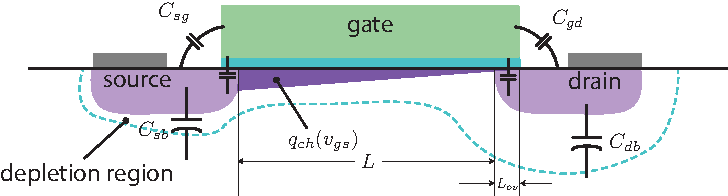
\includegraphics[width=.75\columnwidth]{mos_caps_xsect}
\end{center}
\caption{Cross section of an MOS transistor highlighting the internal capacitance arising from $q_{ch}$ and the parasitic capacitors due to pn-junctions, overlap and fringing capacitance.} \label{fig:moscapsxsect}
\end{figure}

As shown in the device cross-section of Fig.~\ref{fig:moscapsxsect}, MOSFETs have many capacitances. Some critical to the function of the MOS, such as $C_{ox}$, and others are undesired parasitics.  Let us analyze step-by-step where each capacitance comes from.  For now let's ignore the influence of the back gate and just assume the body is AC grounded. In this case, note that channel charge is mostly controlled by gate-source voltage and not the drain voltage.  
%%%%%%%%%%%%%%%%%%%%%%%%%%%%%%%%%%%%%%%%%%%%
%             SUBSECTION 10.2.2            %
%%%%%%%%%%%%%%%%%%%%%%%%%%%%%%%%%%%%%%%%%%%%
\subsection{Gate-Source Capacitance $C_{gs}$}
%%%%%%%%%%%%%%%%%%%%%%%%%%%%%%%%%%%%%%%%%%%%
%                 FIGURE                   %
%%%%%%%%%%%%%%%%%%%%%%%%%%%%%%%%%%%%%%%%%%%%
\begin{figure}[tb]
\begin{center}
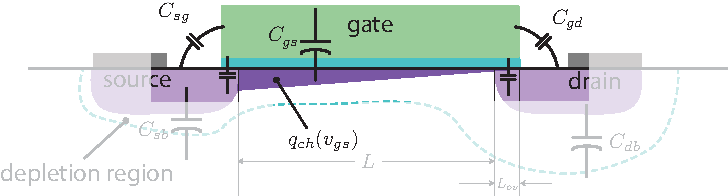
\includegraphics[width=.75\columnwidth]{mos_caps_Cgs}
\end{center}
\caption{The gate-source capacitance is made of two parts; the inversion charge $q_{ch}(v_{gs})$ which is part of the MOS-C internal structure and depends on $C_{ox}$, and other parasitic capacitors.} \label{fig:mos_caps_Cgs}
\end{figure}

Since the drain is isolated from the channel (in saturation), the oxide capacitance $C_{ox}$ is formed from the gate to source, as shown in Fig.~\ref{fig:mos_caps_Cgs}.  But since the inversion charge is "wedge" shaped (inversion decreases as we travel from the source to drain), the effective capacitance is lower.  A detailed calculation shows that
\begin{equation}
	C_{gs} = \frac{2}{3} W L C_{ox} + C_{ov} 
\end{equation} 
We include a parasitic overlap capacitance $C_{ov}$ along source edge of gate 
\begin{equation}
	C_{ov} = L_{ov} W C_{ox}
\end{equation}
The physical origin of the overlap capacitance is the overlap between the gate and the source, resulting from imperfect alignment between the gate and the source, and a diffusion region that grows under the gate.   In a ``good" transistor, $L_{ov} \ll L$, so $C_{gd} \ll C_{gs}$.  The actual value is higher due to fringing fields that leak from the gate to the top of the source and drain junctions.
%%%%%%%%%%%%%%%%%%%%%%%%%%%%%%%%%%%%%%%%%%%%
%             SUBSECTION 10.2.3            %
%%%%%%%%%%%%%%%%%%%%%%%%%%%%%%%%%%%%%%%%%%%%
\subsection{Gate-Drain Capacitance $C_{gd}$}
%%%%%%%%%%%%%%%%%%%%%%%%%%%%%%%%%%%%%%%%%%%%
%                 FIGURE                   %
%%%%%%%%%%%%%%%%%%%%%%%%%%%%%%%%%%%%%%%%%%%%
\begin{figure}[b]
\begin{center}
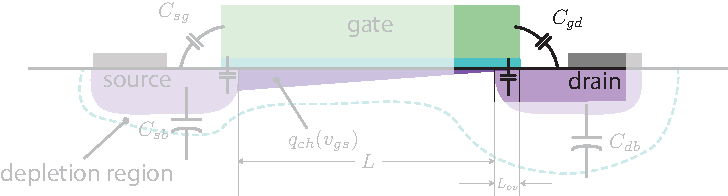
\includegraphics[width=.75\columnwidth]{mos_caps_Cgd}
\end{center}
\caption{The gate-drain capacitance is a parasitic capacitance due to oxide/drain diffusion overlap and fringing terms shown.}
\label{fig:mos_caps_Cgd}
\end{figure}

\begin{equation}
	C_{gd} = C_{ov} + C_{\text{fringe}} = L_{ov} W C_{ox} + C_{\text{fringe}}
\end{equation}
Focusing now on the drain side, Fig.~\ref{fig:mos_caps_Cgd}, we see that the same overlap occurs on the drain side.  Since the MOSFET drain and source are physically identical, this is not surprising\footnote{Some special devices use asymmetric source/drain junctions.}.  Just keep in mind that this capacitance is not due to change in inversion charge in channel.
%%%%%%%%%%%%%%%%%%%%%%%%%%%%%%%%%%%%%%%%%%%%
%             SUBSECTION 10.2.4            %
%%%%%%%%%%%%%%%%%%%%%%%%%%%%%%%%%%%%%%%%%%%%
\subsection{Drain/Source-Bulk Capacitances $C_{db}$ and $C_{sb}$}
The Drain-Bulk and Source-Bulk capacitance is caused by p-n junction depletion regions that isolate the drain/source from the body. The junction forms a ``box" inside the body, and so there are five junctions to consider. Four side-wall junctions and a bottom wall junction, shown in Fig.~\ref{fig:cap_junc_3d}.  The capacitance is defined in terms of the junction areas $A_{s,j}$ and $A_{d,j}$ and the junction perimeters, $P_{s,j}$ and $P_{d,j}$.  As shown in  Fig.~\ref{fig:mos_layout_top}, besides the transistor $L$ and $W$ parameters, we need to know the length of the source and drain diffusion regions, $L_j$, to calculate the area and perimeter.  The junction area is simply $L_j \cdot W$ whereas the perimeter is $(2\cdot L_j + W)$, because the inner junction facing the channel is isolated from the bulk.
\begin{equation}
   C_{sb} = \frac{C_{j0}}{\sqrt{ 1 + V_{SB}/|\phi_{p}}}  A_{s,j} + \frac{C_{j,sw0}}{\sqrt{ 1 + V_{SB}/|\phi_p|}} P_{s,j}
\end{equation}
\begin{equation}
   C_{db} = \frac{C_{j0}}{\sqrt{ 1 + V_{DB}/|\phi_{p}}}  A_{d,j} + \frac{C_{j,sw0}}{\sqrt{ 1 + V_{DB}/|\phi_p|}} P_{d,j}
\end{equation}
Although we have used a grading coefficient of $1/2$ for junctions (leading to square roots in the denominator), in reality this is a parameter that you will adjust based on process parameters.
%%%%%%%%%%%%%%%%%%%%%%%%%%%%%%%%%%%%%%%%%%%%
%                 FIGURE                   %
%%%%%%%%%%%%%%%%%%%%%%%%%%%%%%%%%%%%%%%%%%%%
\begin{figure}[tb]
\begin{center}
\subcaptionbox{\label{fig:cap_junc_3d}}{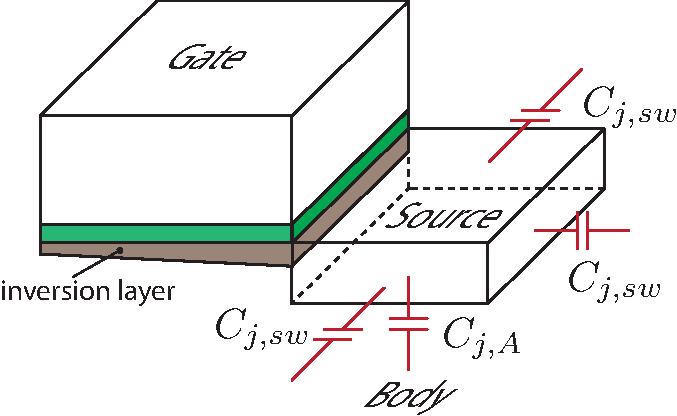
\includegraphics[width=.5\columnwidth]{cap_junc_3d}}
\subcaptionbox{\label{fig:mos_layout_top}}{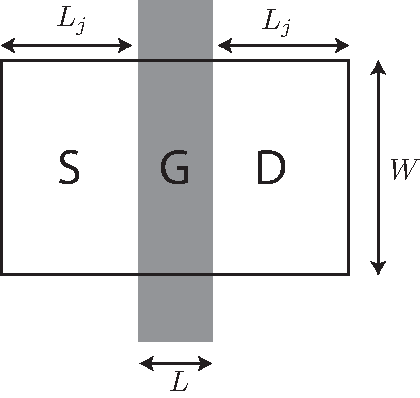
\includegraphics[width=.3\columnwidth]{mos_layout_top}}
\end{center}
\caption{(a) The drain/source junctions form pn-junctions with the body.  Under normal operating conditions, these capacitors are reverse biased.  There are ``sidewall" contributions $C_{j,sw}$ shown and a bottom plate term $C_{j,A}$.  (b)  The junction perimeter and area is calculated from the MOS layout and depends on the width $W$ of the device in addition to the length of the junctions $L_j$.} 
\end{figure}

It's important to realize that the source/drain are symmetric.  The source / drain is defined by potentials / biasing and the schematic rather than the process. For this reason, the doping parameters for the source and drain are symmetric and so the calculations for the source and drain to bulk are very much the same.  Of course, the area of the junctions may differ based on the device layout.	Some special technologies (high breakdown devices) have an asymmetric source/drain, but this is rare.	 If the source and body are both AC grounded, then the source-to-bulk capacitance does not play a role in AC response and it's excluded from the model.
%%%%%%%%%%%%%%%%%%%%%%%%%%%%%%%%%%%%%%%%%%%%
%             SUBSECTION 10.2.5            %
%%%%%%%%%%%%%%%%%%%%%%%%%%%%%%%%%%%%%%%%%%%%
\subsection{Three Terminal Small Signal Model Including Capacitors}
%%%%%%%%%%%%%%%%%%%%%%%%%%%%%%%%%%%%%%%%%%%%
%                 FIGURE                   %
%%%%%%%%%%%%%%%%%%%%%%%%%%%%%%%%%%%%%%%%%%%%
\begin{figure}[tb]
\begin{center}
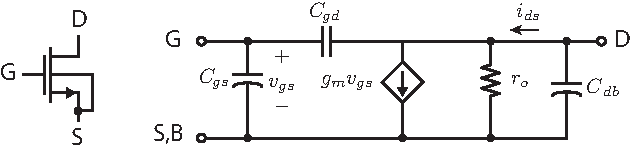
\includegraphics[scale=1]{mos3term_ac}
\end{center}
\caption{The complete three terminal model of a MOSFET with source-body tied together includes  capacitance $C_{gs}$ and the parasitic $C_{gd}$ and $C_{db}$.}
\label{fig:mos3term_ac}
\end{figure}

We can now update our three-terminal small-signal model to include three capacitors, as shown in Fig.~\ref{fig:mos3term_ac}.  The capacitance $C_{gs}$ is a combination of the gate-oxide capacitance (recall the factor of $2/3$ arising from the uneven charge distribution in the saturation region), and any overlap and fringing capacitance between the gate and the source.  The capacitance $C_{gd}$, on the other hand, is all due to overlap since in the saturation region the drain is isolated from the channel due to pinch-off.  The capacitance $C_{db}$ simply accounts for the reverse-biased pn-junction capacitance from the drain diffusion region to the body of the transistor.  The capacitor $C_{sb}$ is missing from the model because it's shorted out in the three terminal model if we assume the source/bulk are tied together.  In practice, this may not be true and we should include this capacitor as well, as we'll discuss in the full four-terminal model.  
%%%%%%%%%%%%%%%%%%%%%%%%%%%%%%%%%%%%%%%%%%%%%%%%%%%%%%%%%%%%%%%%%%%%%%%%%%%%%%%%%%%%%%%%
%%%%%%%%%%%%%%%%%%%%%%%%%%%%%%%%%%%%%%%%%%%%%%%%%%%%%%%%%%%%%%%%%%%%%%%%%%%%%%%%%%%%%%%%
%                                   SECTION 10.3                                       %
%%%%%%%%%%%%%%%%%%%%%%%%%%%%%%%%%%%%%%%%%%%%%%%%%%%%%%%%%%%%%%%%%%%%%%%%%%%%%%%%%%%%%%%%
%%%%%%%%%%%%%%%%%%%%%%%%%%%%%%%%%%%%%%%%%%%%%%%%%%%%%%%%%%%%%%%%%%%%%%%%%%%%%%%%%%%%%%%%
\section{Back-Gate Effect}
%%%%%%%%%%%%%%%%%%%%%%%%%%%%%%%%%%%%%%%%%%%%
%             SUBSECTION 10.3.1            %
%%%%%%%%%%%%%%%%%%%%%%%%%%%%%%%%%%%%%%%%%%%%
\subsection{All MOSFETS have a ``Back Door"}
%%%%%%%%%%%%%%%%%%%%%%%%%%%%%%%%%%%%%%%%%%%%
%                 FIGURE                   %
%%%%%%%%%%%%%%%%%%%%%%%%%%%%%%%%%%%%%%%%%%%%
\begin{figure}[b]
\begin{center}
\subcaptionbox{\label{fig:mos4term}}{
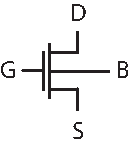
\includegraphics[width=.15\columnwidth]{mos4term}}
\subcaptionbox{\label{fig:mos_backgate}}{
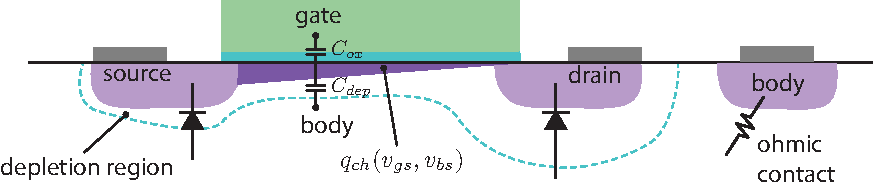
\includegraphics[width=.75\columnwidth]{mos_backgate}}
\end{center}
\caption{The body terminal of a MOSFET is an independent fourth terminal of the device.  Variations in the body voltage couple into the channel charge through $C_{dep}$, in a similar manner as gate voltage variations couple into the channel charge through $C_{gs}$. } 
\end{figure}

So far we have been ignoring the body terminal of the device, shown explicitly in Fig.~\ref{fig:mos4term}.  The MOS transistor has some symmetry that you should appreciate between the source and drain.  It's less obvious, but there is a symmetry between the gate and the body if you think about how the inversion charge depends on both voltages. We will show that the body can act like a ``back gate" and control the inversion and thus the current in the device, as shown in Fig.~\ref{fig:mos_backgate}.  It's something we've ignored because in many instances the body terminal is simply tied to the source, and the source is sometimes at ground or $V_{SS}$ for NMOS, or supply or $V_{DD}$ for PMOS.  What we'd like to understand is what happens if there is a DC voltage or an AC voltage swing on the body terminal.
%%%%%%%%%%%%%%%%%%%%%%%%%%%%%%%%%%%%%%%%%%%%
%             SUBSECTION 10.3.2            %
%%%%%%%%%%%%%%%%%%%%%%%%%%%%%%%%%%%%%%%%%%%%
\subsection{Body Bias Affects $V_T$ - DC Signals}
From our calculations of the MOS capacitor, we know that the body bias $V_{SB}$ has an impact on the channel charge.  There is a depletion capacitance between the transistor body and the channel:
\begin{equation}
	{C_{dep}} = {\varepsilon _s}/{x_{dep,\max }}
\end{equation}
If we take into account the body voltage with respect to the source, the amount of inversion charge is given by
\begin{equation}
	{Q_{inv}} =  - {C_{ox}}({V_{GS}} - {V_T}) - {C_{dep}}{V_{BS}}
\end{equation}
Here the role of the back-gate is shown explicitly and symmetrically with respect to the front gate.  Whereas the front gate, or simply the gate, affects the inversion charge through $C_{ox}$, the back-gate affects the amount of inversion charge through $C_{dep}$.  
%
Let's factor out $C_{ox}$ and note that $V_{SB} = - V_{BS}$:
\begin{equation}
	{Q_{inv}} =  - {C_{ox}}\left[ {{V_{GS}} - {V_T} + \frac{{{C_{dep}}}}{{{C_{ox}}}}{V_{SB}}} \right]
\end{equation}
Written in this form, we can lump the back-gate effect into a change in the threshold voltage:
\begin{equation}
	{V_T}({V_{SB}}) = {V_{T0}} + \frac{{{C_{dep}}}}{{{C_{ox}}}}{V_{SB}}
\end{equation}
where $V_{T0}$ is the zero $V_{SB}$ threshold voltage:
\begin{equation}
{V_{T0}} = {V_T}(0) = {V_{FB}} - 2{\phi _p} + \frac{1}{{{C_{ox}}}}\sqrt {2q{\varepsilon _s}{N_a}( - 2{\phi _p})} 
\end{equation}
and the change in threshold due to body bias is given by
\begin{equation}
	\Delta {V_T} = \frac{1}{{{C_{ox}}}}\sqrt {2q{\varepsilon _s}{N_a}} \left(\sqrt { - 2{\phi _p} + {V_{SB}}}  - \sqrt { - 2{\phi _p}} \right) = \gamma \left( {\sqrt {{V_{SB}} - 2{\phi _p}}  - \sqrt { - 2{\phi _p}} } \right)
\end{equation}
This is written more compactly in the following form:
\begin{equation}
	{V_T} = {V_{T0}} + \gamma \left( {\sqrt {{V_{SB}} - 2{\phi _p}}  - \sqrt { - 2{\phi _p}} } \right)
	\label{eq:vtbias}
\end{equation}
where $\gamma$ is a device parameter
\begin{equation}
	\gamma = \frac{\sqrt{2q\varepsilon_s N_a}}{C_{ox}}
\end{equation}
%%%%%%%%%%%%%%%%%%%%%%%%%%%%%%%%%%%%%%%%%%%%
%             SUBSECTION 10.3.3            %
%%%%%%%%%%%%%%%%%%%%%%%%%%%%%%%%%%%%%%%%%%%%
\subsection{Role of the Substrate Potential - AC Signals}
Since $V_{SB}$ changes the threshold voltage, which in turn changes the drain current, the body acts like a ``back-gate” and it should cause an AC current to flow in response to an AC signal between the body and source.  The back-gate transconductance is defined as:
\begin{equation} 
	{g_{mb}} = {\left. {\frac{{\Delta {i_D}}}{{\Delta {v_{BS}}}}} \right|_Q} = {\left. {\frac{{\partial {i_D}}}{{\partial {v_{BS}}}}} \right|_Q} 
\end{equation}
We can simplify this calculation by using the chain rule and taking advantage of our previous calculation of the change in $V_T$:
\begin{equation}
	{g_{mb}} = {\left. {\frac{{\partial {I_D}}}{{\partial {V_{BS}}}}} \right|_Q} = {\left. {\frac{{\partial {I_D}}}{{\partial {V_{T}}}}} \right|_Q}{\left. {\frac{{\partial {V_{T}}}}{{\partial {V_{BS}}}}} \right|_Q}
\end{equation}
We have that the threshold voltage is given by Eq.~\ref{eq:vtbias}.  Taking the derivatives with $V_{BS}$ and $V_T$ results in the following:
\begin{equation}
	{g_{mb}} = {\left. {\frac{{\partial {I_D}}}{{\partial {V_{BS}}}}} \right|_Q} 
= {\left. {\frac{{\partial {I_D}}}{{\partial {V_{T}}}}} \right|_Q}{\left. {\frac{{\partial {V_{T}}}}{{\partial {V_{BS}}}}} \right|_Q} = \frac{{\gamma {g_m}}}{{2\sqrt { - {V_{BS}} - 2{\phi _p}} }}
\end{equation}
You can also intuitively guess that the answer should in fact be equal to:
\begin{equation}
	g_{mb} = g_m \frac{C_{dep}}{C_{ox}}
\end{equation}
In most transistors $C_{ox} > C_{dep}$, so the back-gate transconductance is smaller.   
%%%%%%%%%%%%%%%%%%%%%%%%%%%%%%%%%%%%%%%%%%%%%%%%%%%%%%%%%%%%%%%%%%%%%%%%%%%%%%%%%%%%%%%%
%%%%%%%%%%%%%%%%%%%%%%%%%%%%%%%%%%%%%%%%%%%%%%%%%%%%%%%%%%%%%%%%%%%%%%%%%%%%%%%%%%%%%%%%
%                                   SECTION 10.4                                       %
%%%%%%%%%%%%%%%%%%%%%%%%%%%%%%%%%%%%%%%%%%%%%%%%%%%%%%%%%%%%%%%%%%%%%%%%%%%%%%%%%%%%%%%%
%%%%%%%%%%%%%%%%%%%%%%%%%%%%%%%%%%%%%%%%%%%%%%%%%%%%%%%%%%%%%%%%%%%%%%%%%%%%%%%%%%%%%%%%
\section{Complete Four Terminal MOS Small-Signal Model}
%%%%%%%%%%%%%%%%%%%%%%%%%%%%%%%%%%%%%%%%%%%%
%             SUBSECTION 10.4.1            %
%%%%%%%%%%%%%%%%%%%%%%%%%%%%%%%%%%%%%%%%%%%%
\subsection{Four-Terminal Small-Signal Model}
%%%%%%%%%%%%%%%%%%%%%%%%%%%%%%%%%%%%%%%%%%%%
%                 FIGURE                   %
%%%%%%%%%%%%%%%%%%%%%%%%%%%%%%%%%%%%%%%%%%%%
\begin{figure}[tb]
\begin{center}
\subcaptionbox{\label{fig:mos4term_dc_gmb}}{
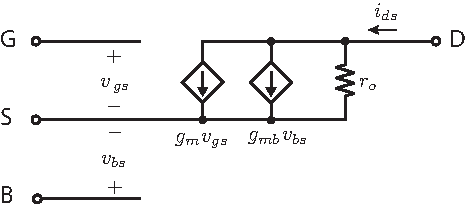
\includegraphics[scale=.9]{mos4term_dc_gmb}}
\subcaptionbox{\label{fig:mos4term_ac_gmb}}{
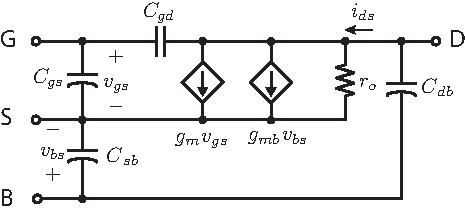
\includegraphics[scale=.9]{mos4term_ac_gmb}}
\end{center}
\caption{The complete small-signal models for an n-type MOSFET with (a) no capacitors and with (b) capacitors.  The model without capacitors is useful for low frequency calculations.} 
\end{figure}

We now complete the small-signal model by noting that the drain-source current depends on $v_{gs}$ (transconductance), on $v_{ds}$ (output resistance of device), and also on $v_{bs}$ (back-gate):
\begin{equation}
	{i_{ds}} = {g_m}{v_{gs}} +  \frac{1}{{{r_o}}}{v_{ds}} + {g_{mb}}{v_{bs}} 
\end{equation}
This equation is captured by the equivalent circuit shown in Fig.~\ref{fig:mos4term_dc_gmb}.  This model naturally shows the symmetry between the front-gate and the back-gate.  If we include all the capacitors as well, we arrive at Fig.~\ref{fig:mos4term_ac_gmb}, the complete small-signal model for an NMOS transistor.
%%%%%%%%%%%%%%%%%%%%%%%%%%%%%%%%%%%%%%%%%%%%
%             SUBSECTION 10.4.2            %
%%%%%%%%%%%%%%%%%%%%%%%%%%%%%%%%%%%%%%%%%%%%
\subsection{Complete Small-Signal Model PMOS}
Using the same arguments, we can also conclude that a PMOS device is also described by a similar four terminal small-signal equivalent circuit model, as shown in Fig.~\ref{fig:pmos4term_ac}.
%%%%%%%%%%%%%%%%%%%%%%%%%%%%%%%%%%%%%%%%%%%%
%                 FIGURE                   %
%%%%%%%%%%%%%%%%%%%%%%%%%%%%%%%%%%%%%%%%%%%%
\begin{figure}[h]
\begin{center}
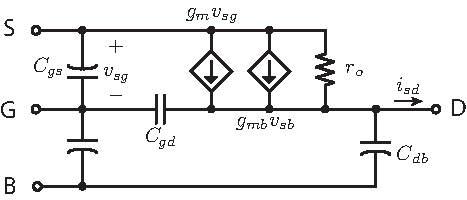
\includegraphics[scale=1]{pmos4term_ac}
\end{center}
\caption{The complete small-signal models for an p-type MOSFET.}
\label{fig:pmos4term_ac}
\end{figure}
